\documentclass[a4paper]{scrartcl}

\usepackage[T1]{fontenc}
\usepackage[utf8]{inputenc}

\title{The TTC 2019 TT2BDD Case}
\author{
  Antonio García-Domínguez\\
  Aston University\\
  B4 7ET, Birmingham, United Kingdom\\
  a.garcia-dominguez@aston.ac.uk
}

\usepackage{tikz}
\usepackage{graphicx}
\graphicspath{{}{figures/}}

\usepackage[pdftex,colorlinks=true]{hyperref}

\usepackage{listings}
\lstset{columns=flexible}

\newcommand*{\class}[1]{\textsc{#1}}
\newcommand*{\feature}[1]{\emph{#1}}
\newcommand*{\file}[1]{\texttt{#1}}

\begin{document}

\maketitle

\begin{abstract}
  Model transformation tools have reached a considerable level of maturity in
  the core features, and are currently developing in many directions. Some tools
  are focusing on providing higher performance for large models or complex
  transformations. Others focus on bidirectionality, visualisation,
  traceability, or verifiability, among other research directions. Whereas past
  cases in TTC have focused on specific research directions, this case study
  presents a well-known simple transformation and welcomes researchers to apply
  their research to it. The aim of this case is to serve as a showcase of the
  various directions that model transformation research is going towards at the
  moment.
\end{abstract}

\section{Introduction}

Past editions of the Transformation Tool Contest have focused on a variety of
topics:
\begin{itemize}
\item In 2018, the Quality-based Software Selection and Hardware-Mapping
  case~\cite{gotz_quality-based_2018} discussed optimisation-oriented model
  transformations (with a combination of performance and solution quality). The
  Social Media Live Case~\cite{hinkel_ttc_2018} considered performance in
  updating model views as models changed (with a strong preference for
  approaches supporting incrementality).

\item In 2017, the Smart Grid case focused on
  incrementality~\cite{hinkel_ttc_2017}, the Families to Persons case discussed
  bidirectional transformations~\cite{anjorin_families_2017}, State Elimination
  focused on performance and the live case on Transformation
  Reuse~\cite{live2017} discussed mechanisms to share complex logic across
  multiple versions of a transformation.

\item In 2016, optimisation-oriented model transformations were discussed in
  considerable breadth through the Class Responsibility Assignment
  case~\cite{fleck_class_2016}, and an alternative dataflow-based notation for
  model transformation was evaluated in the live case study~\cite{live2016}.
\end{itemize}

While these were notable examples of realistic transformations, they were
narrowly focused on a specific topic,and their inherent complexity discouraged
some attendees from trying their hand with their own research agenda on the
transformation.

This year, we propose a broader contest that welcomes all active lines of work
on model transformation. It is based on a simpler, well-known transformation
from the ATL Zoo~\cite{atlzoo}: TT2BDD (Truth Tables to Binary Decision
Diagrams). Striving for raw performance is an option, but the case welcomes
approaches that focus on other attributes of interest of a high-quality model
transformation: for example, verifiability, traceability, bidirectionality, or
understandability. Solution providers are welcome to propose their own
attributes of interest. In general, this case is proposed as a showcase of the
current variety of model transformation tools.

All resources for this case are available on
Github\footnote{\url{https://github.com/TransformationToolContest/ttc2019-tt2bdd}}.
Please follow the link in the footnote and create a pull request with your own
solution after you have submitted your description to EasyChair.

The rest of the document is structured as follows:
Section~\ref{sec:transf-descr} describes the TT2BDD transformation.
Section~\ref{sec:task-suggestions} several tasks of interest that
should be tackled in a solution (authors are free to propose their own tasks of
interest). Section~\ref{sec:benchmark-framework} mentions the benchmark
framework for those solutions that focus on raw performance. Finally,
Section~\ref{sec:evaluation} mentions an outline of the initial audience-based
evaluation across all solutions, and the approach that will be followed to
derive additional prizes depending on the attributes targeted by the solutions.

\section{Transformation Description}
\label{sec:transf-descr}

This section introduces the Truth Tables to Binary Decision Diagram
transformation, with a description of the input and output metamodels, and an
outline of an implementation.

\subsection{Input Metamodel: Truth Tables}
\label{sec:input-metam-truth}

\begin{figure}
  \centering
  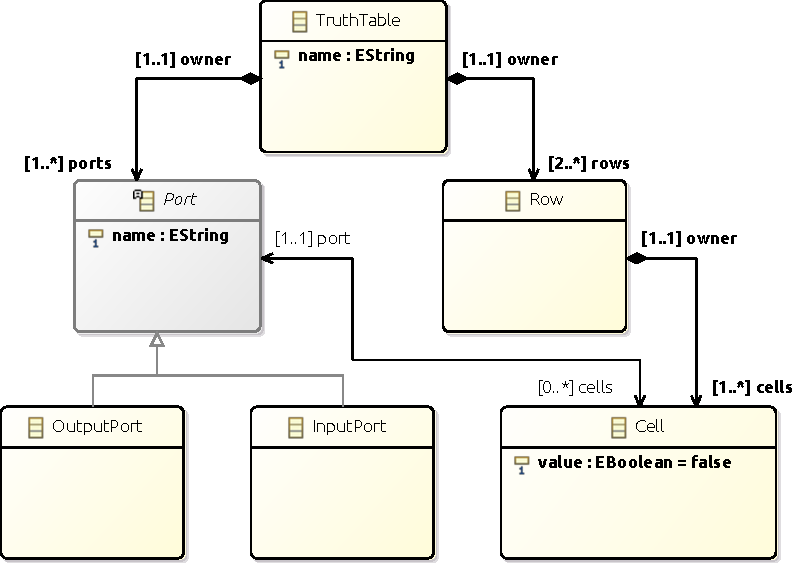
\includegraphics[width=.9\textwidth]{tt}
  \caption{Class diagram for the input Truth Tables metamodel}
  \label{fig:tt-metamodel}
\end{figure}

\begin{table}
  \centering
  \begin{tabular}{llll|l}
    $A$ & $B$ & $C$ & $D$ & $S$ \\
    \hline
    0 & 0 & - & - & 0 \\
    0 & 1 & 0 & 0 & 1 \\
    0 & 1 & 0 & 0 & 1 \\
    0 & 1 & 0 & 1 & 0 \\
    0 & 1 & 1 & - & 0 \\
    1 & 0 & 0 & 0 & 0 \\
    1 & 0 & 1 & 0 & 1 \\
    1 & - & - & 1 & 0 \\
    1 & 1 & 0 & 0 & 1 \\
    1 & 1 & 1 & 0 & 0 \\
  \end{tabular}
  \caption{Example truth table: $A$ to $D$ are input ports and $S$ is an output port. ``-'' means ``ignored''.}
  \label{tab:tt-example}
\end{table}

The input metamodel is shown on Figure~\ref{fig:tt-metamodel}. The
\class{Truth\-Table} class is as the root of the model, and contains a
collection of \class{Port}s and \class{Row}s. \class{Port}s come in two types:
\class{Input\-Port}s and \class{Output\-Port}s. \class{Row}s contain sequences
of \class{Cell}s, which assign values to the \class{Input\-Port}s and
\class{Output\-Port}s of the table.

Automated EMF opposite references are used liberally in the metamodel to
simplify the specification of the transformation. \feature{owner} is used to
access the container from several child objects (e.g. the \class{Truth\-Table}
of a \class{Row}), and it is possible to see which \feature{cells} referenced a
specific \class{Port}.

A sample model is shown on Table~\ref{tab:tt-example}. The truth table has four
\class{Input\-Port}s named $A$ to $D$, and one \class{Output\-Port} named $S$.
The first \class{Row} contains only 3 \class{Cell}s, specifying that if $A$ and
$B$ are 0, then $S$ should be 0.

\subsection{Output Metamodel: Binary Decision Trees}
\label{sec:outp-metam-binary}

\begin{figure}
  \centering
  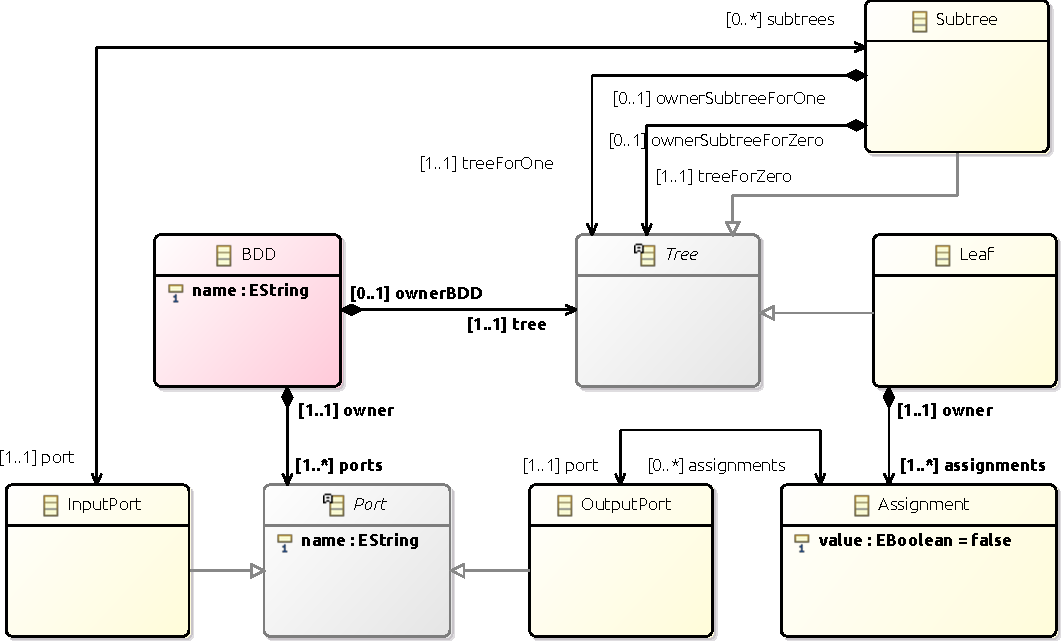
\includegraphics[width=.9\textwidth]{bdd}
  \caption{Class diagram for the output Binary Decision Diagram metamodel}
  \label{fig:bdd-metamodel}
\end{figure}

\begin{figure}
  \centering
  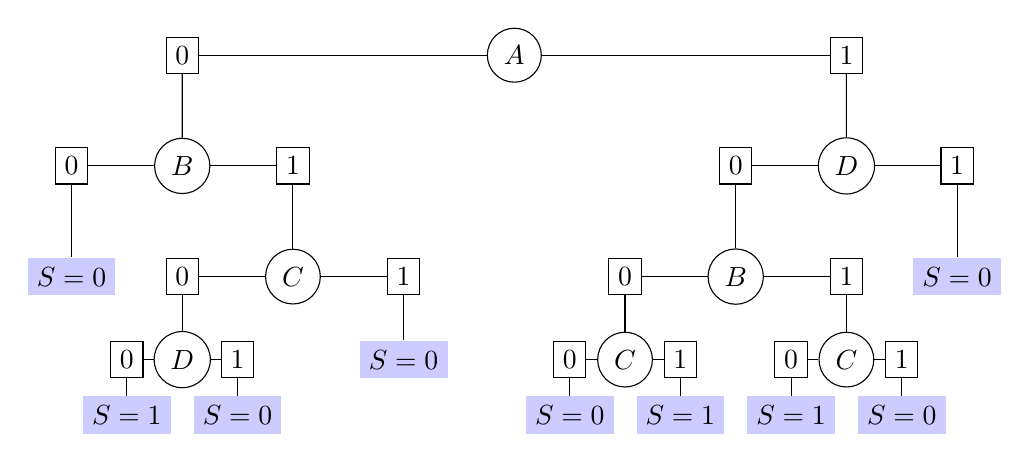
\begin{tikzpicture}[
      level 1/.style={level distance=12em},
      level 2/.style={level distance=4em},
      level 6/.style={level distance=3em},
      level 7/.style={level distance=2em},
      port/.style={circle, draw},
      value/.style={draw},
      assignment/.style={fill=blue!20},
  ]
    \node[port] {$A$}
    child[grow=left] {
      node[value] {0}
      [grow=down]
      child {
        node[port] {$B$}
        child[grow=left] {
          node[value] {0}
          child[grow=down] { node[assignment] {$S = 0$} }
        }
        child[grow=right] {
          node[value] {1}
          child[grow=down] {
            node[port] {$C$}
            child[grow=left] {
              node[value] {0}
              child[grow=down] {
                node[port] {$D$}
                child[grow=left] {
                  node[value] {0}
                  child[grow=down] { node[assignment] {$S=1$} }
                }
                child[grow=right] {
                  node[value] {1}
                  child[grow=down] { node[assignment] {$S=0$} }
                }
              }
            }
            child[grow=right] {
              node[value] {1}
              child[grow=down] {node[assignment] {$S=0$}}
            }
          }
        }
      }
    }
    child[grow=right] {
      node[value] {1}
      [grow=down]
      child {
        node[port] {$D$}
        child[grow=left] {
          node[value] {0}
          child[grow=down] {
            node[port] {$B$}
            child[grow=left] {
              node[value] {0}
              child[grow=down] {
                node[port] {$C$}
                child[grow=left] {
                  node[value] {0} child[grow=down] { node[assignment] {$S=0$} }
                }
                child[grow=right] {
                  node[value] {1} child[grow=down] { node[assignment] {$S=1$} }
                }
              }
            }
            child[grow=right] {
              node[value] {1}
              child[grow=down] {
                node[port] {$C$}
                child[grow=left] {
                  node[value] {0} child[grow=down] { node[assignment] {$S=1$} }
                }
                child[grow=right] {
                  node[value] {1} child[grow=down] { node[assignment] {$S=0$} }
                }
              }
            }
          }
        }
        child[grow=right] {
          node[value] {1} child[grow=down] { node[assignment] {$S=0$} }
        }
      }
    }
    ;
  \end{tikzpicture}
  \caption{Equivalent BDD for the truth table on Table~\ref{tab:tt-example}}
  \label{fig:bdd-equivalent}
\end{figure}

The output metamodel is shown on Figure~\ref{fig:bdd-metamodel}. The \class{BDD}
class is the root of the model, and contains the root of the \class{Tree}
and a collection of \class{Port}s. Similarly to the Truth Tables metamodel,
there are \class{Input\-Port}s and \class{Output\-Port}s.

\class{Tree} is the common superclass for any node in the tree. Inner nodes
check the value of an \class{Input\-Port}: if it is a false value, evaluation
will proceed through the \feature{tree\-For\-Zero} \class{Tree}; otherwise,
evaluation will go through the \feature{tree\-For\-One} \class{Tree}. Leaf nodes
are \class{Leaf} objects, which provide an \class{Assignment} of a boolean value
to each of the available \class{Output\-Port}s.

The equivalent BDD for the truth table on Table~\ref{tab:tt-example} is shown on
Figure~\ref{fig:bdd-equivalent}. \class{Subtree}s are represented by the circle
referencing an \class{Input\-Port} and their subtrees for when the port takes a
0 or 1 value. \class{Assignment}s are represented by the highlighted nodes that
provide values to the \class{Output\-Port}s.

\subsection{Process Outline}
\label{sec:process-outline}

The transformation essentially needs to construct a (preferably minimal) binary
decision diagram that produces the same values for the output ports, given the
same values in the input ports. Given the high interest about this problem in
circuit design, many algorithms have been proposed in the literature.

Solution authors are welcome to implement a more optimal algorithm in their
transformation tool. This section will only outline a simple approach that can
be readily implemented without too much complication.

There are some basic mappings which are immediately obvious:

\begin{itemize}
\item Each \class{TruthTable} object should correspond to a \class{BDD} object,
  with the same name and equivalent \class{Port}s.

\item Each \class{Input\-Port} and \class{Output\-Port} should be mapped to an
  object of the BDD type with the same name, and should be assigned the same
  \feature{name}.

\item Each \class{Row} should become a \class{Leaf} node: the \class{Cell}s for
  the \class{Output\-Port}s will become \class{Assignment}s.
\end{itemize}

The complexity is in deriving the inner nodes: the \class{Subtree} objects. One
simple approach is to find a TT \class{Input\-Port} which is (ideally) defined
in all the \class{Row}s, and turn it into an inner node (a \class{Subtree})
which points to the equivalent BDD \class{Input\-Port} and has two
\class{Tree}s:
\begin{itemize}
\item The zero subtree, produced from the \class{Row}(s) where the port was 0.
  This will be a \class{Subtree} if there are at least two rows in that
  situation: the transformation should proceed recursively in this case with
  those rows, excluding the input ports that have already been considered. If
  there is only one such row, this would simply point to the \class{Leaf}
  created above.

\item The one subtree, produced in a parallel way to the zero subtree.
\end{itemize}

This simple approach does not necessarily ensure a minimal subtree, as in some
points there may be multiple ports to choose from. It may require improvements
for cases where there are no input ports which are defined in all available
rows. Authors are welcome to implement a more efficient or optimal approach in
their solutions.

\section{Main Task}
\label{sec:task-suggestions}

The obvious main task in this case is to implement the TT2BDD transformation in
your favourite model transformation language, ensuring that the resulting BDDs
are equivalent to the original truth table. To simplify the work involved, the
case includes an Eclipse Modelling Framework implementation of the metamodels in
the \file{ttc2019.metamodels} project within the \file{metamodels} folder, and a
set of sample XMI input models conforming to the metamodels in the \file{models}
folder.

The \file{models} folder includes two additional tools, which can be run with
\file{java -jar tool.jar}:
\begin{itemize}
\item \file{generator.jar} can produce truth tables of an arbitrary number of
  input and output ports, given seed. Solution implementers may want to be
  careful with the values given, as truth tables grow exponentially as more
  input ports are added.

\item \file{validator.jar} can validate if a BDD model is equivalent to a source
  truth table model, by evaluating all the rows in the TT model through the BDD
  and comparing the values of the \class{Output\-Port}s. This tool is required
  to check that your transformation is correct.
\end{itemize}

Solutions are free to focus on any specific quality attribute of the
transformation beyond optimality and performance. For instance, it may be useful
to be able to prove that the transformation does indeed produce a BDD which is
equivalent to the TT (even if suboptimal). It may also be interesting to be able
to visualize the BDD being built from the TT, or to be able to trace which
subtree came from which collection of rows.

The conciseness of the transformation may also be of interest, given that its
recursive nature may be difficult to map to some existing transformation
languages.

\section{Benchmark Framework}
\label{sec:benchmark-framework}

If focusing on performance, the solution authors should integrate their solution
with the provided benchmark framework. It is based on that of the TTC 2017 Smart
Grid case~\cite{hinkel_ttc_2017}, and supports the automated build and execution
of solutions. For this specific case study, the visualisation of the results is
currently disabled.

The benchmark consists of three phases:

\begin{enumerate}
\item \textbf{Initialization}, which involves setting up the basic
  infrastructure (e.g. loading metamodels). These measurements are optional.
\item \textbf{Load}, which loads the input models.
\item \textbf{Run}, which runs the transformation, produces the BDD and saves
  the file.
\end{enumerate}

\subsection{Solution requirements}
\label{sec:solut-requ}

Solutions should be forks of the main Github
project\footnote{\url{https://github.com/TransformationToolContest/ttc2019-tt2bdd}},
and should be submitted as pull requests after the descriptions have been
submitted to EasyChair. For details about the submission format, please consult
the call for
solutions\footnote{\url{https://www.transformation-tool-contest.eu/cfs.html}}.

Each solution wishing to use the benchmarking framework should print to the
standard output a line with the following fields, separated by semicolons
(``;''):

\begin{itemize}
\item \textbf{Tool}: name of the tool.
\item \textbf{Model}: name of the model being transformed.
\item \textbf{RunIndex}: the index of the repetition of the transformation.
\item \textbf{Phase}: the name of the phase.
\item \textbf{MetricName}: the name of the metric. It may be the used
  \textbf{Memory} in bytes, or the wall clock \textbf{Time} spent in integer
  nanoseconds.
\end{itemize}

\lstinputlisting[
  float,frame=tb,numbers=left,
  caption={\file{solution.ini} file for the reference ATL solution},
  label=lst:ini-atl
]{../../solutions/EMFSolutionATL/solution.ini}

To enable automatic execution by the benchmark framework, solutions should add a
subdirectory to the \file{solutions} folder of the benchmark with a
\file{solution.ini} file stating how the solution should be built and how it
should be run. As an example, the \file{solution.ini} file for the reference ATL
solution is shown on Listing~\ref{lst:ini-atl}. In the \file{build} section, the
\file{default} option specifies the command to build and test the solution, and
the \file{skipTests} option specifies the command to build the solution while
skipping unit tests. In the \file{run} section, the \file{cmd} option specifies
the command to run the solution.

The repetition of executions as defined in the benchmark configuration is done
by the benchmark. For 5 runs, the specified command will be called 5 times,
passing any required information (e.g. run index, or input model name) through
environment variables. Solutions must not save intermediate data between
different runs: each run should be entirely independent.

The name and absolute path of the input model, the run index and the name of the
tool are passed using environment variables \file{Model}, \file{ModelPath},
\file{RunIndex} and \file{Tool}. Solution authors are suggested to study the
example ATL solution on how to use these values to run their transformation.

\subsection{Running the benchmark}
\label{sec:running-benchmark}

The benchmark framework only requires Python 3.3 to be installed. Furthermore,
the solutions may imply additional frameworks. We would ask solution authors to
explicitly note dependencies to additional frameworks necessary to run their
solutions.

If all prerequisites are fulfilled, the benchmark can be run using Python with
the command \file{python scripts/run.py}. Additional options can be queried
using the option \file{{-}{-}help}. The benchmark framework can be configured
through the \file{config/config.json} file: this includes the input models to be
evaluated (some of which have been excluded by default due to their high cost with the sample solution), the names of the tools to be run, the number of runs per tool+model, and the timeout for each command in milliseconds.

\section{Evaluation}
\label{sec:evaluation}

Given the call for a broader set of research interests in this transformation,
the evaluation will operate on two dimensions:

\begin{itemize}
\item Is it a high-quality model transformation? The transformation should be
  complete, correct, easy to understand, efficient, and produce optimal results.

  The \file{validator.jar} will be used to check the produced BDDs against the
  source truth tables, and the authors will need to provide a convincing
  argument about the correctness of the solution.

  Attendees to the contest will evaluate the understandability of the solution,
  and the benchmark framework will provide independent measurements of memory
  and time usage.

  Tree sizes for the BDDs will be considered for the optimality of the
  transformations: the smaller, the better.

\item Does it highlight a promising research direction? Although the
  transformation may not be entirely complete or may be harder to understand, it
  may serve as an example of an active research area within model
  transformations that the community may wish to showcase.

  This may include aspects such as incrementality, bidirectionality,
  traceability, verifiability, or the ability to visualize interactively the
  transformation, among other areas of interest in the field.

  Depending on the submitted solutions, the awards for this dimension may
  change. If there are no common areas of interest in the solutions, an
  audience-driven ``Most Promising'' award will be awarded. If there are common
  themes between solutions, dedicated 1st/2nd/3rd place awards for those
  research areas may be awarded.
\end{itemize}

\bibliographystyle{plain}
\bibliography{bibliography}

\end{document}
